Serverless computing (also known as Functions-as-a-Ser\-vice (FaaS))~\cite{ref:aws-lambda,ref:faas3,ref:afunctions-16} is a popular cloud service for hosting and automatically scaling applications. Originally designed for web services~\cite{ref:lambda-webservices,ref:lambda-microservices}, serverless computing defines a simple, event-driven programming model and cloud platform with which developers write simple, short-lived functions that are invoked by the platform in response to specific system-wide events (e.g. storage updates, notifications, messages received, changes in state, custom events, etc.). Serverless platforms automatically configure and provision isolated execution environments (typically via Linux containers) on-demand and users pay only for the resources their functions use during execution. Given its success to date, public cloud providers and open source communities have released multiple serverless platforms with similar functionality~\cite{ref:aws-lambda,ref:afunctions-16,ref:gfunctions-16,cspot19,ref:openwhisk-16,ref:ironio-16}.

Moreover, serverless computing has been extended to work at the ``edge'' of the network to reduce the response latency and bandwidth associated with public cloud use by data-driven applications (e.g.  those that target the Internet of Things (IoT))~\cite{ aws-greengrass, iothub-web, iotedge-web}. Doing so is challenging however, because there is a scarcity of computing and storage resources at the edge relative to resource-rich public and private clouds. Moreover, public/private clouds may offer specialized hardware (e.g. GPUs) that can significantly speed up machine learning applications, which is not commonly available in resource-restricted edge clouds.

In this paper, we investigate the use of serverless computing across the edge and public cloud deployments (hybrid cloud settings). We develop a scheduling system, called the Serverless TeleOperable Hybrid Cloud (STOIC), which automatically places and deploys functions across these systems aiming to reduce the total execution time latency (versus using either system in isolation). We specifically target image-based, object recognition using Tensorflow (for training and inference) in this work.

\iffalse
In particular, we couple edge systems without GPUs with public (shared) cloud systems with GPUs. Moreover, we do so for an important class of machine learning applications -- those that perform model training (versus inference or classifications), given that much past work has argued that training should not be performed at the edge due to limited resources and lack of acceleration~\cite{ref:dependability}.
\fi

STOIC automatically places serverless functions at the edge (without GPUs) or in public cloud instances (equipped with 1+ GPUs) using predicted latency.
We use the system to perform online training and inference for batches of images from motion-triggered, camera traps that capture images of wildlife in a remote locations, with intermittent Internet connectivity.

% removed for blind review at Sedgwick Research
%Reserve~\cite{ref:sedgwick}. 

STOIC has two placement scenarios: the first places functions only at the runtime with the least predicted latency, whereas the second places functions concurrently at both edge and public cloud, but then terminates public cloud execution if/when it determines that the edge will finish sooner. The former scenario is called \textit{Selector} mode. The latter scenario, called \textit{Duplicator} mode, is useful when the cloud and/or network performance used for deployment is intermittent or highly variable, or when executing at the edge incurs no cost or other penalty -- to ensure that progress is made. Our results show that STOIC speeds up the total response time of the application by 3.3x versus a baseline scenario. In selector mode, STOIC achieves a placement accuracy of 92\% relative to the optimal placement.  In duplicator mode, STOIC accuracy is 95\% for 2 GPUs and 97\% (versus optimal) for 1 GPU cloud deployments over a 24 hour period.


\iffalse
To do so, STOIC estimates, using execution histories, transfer time (for sending image batches to the public cloud), deployment time (to spin up runtime containers in the public cloud), and execution time (for executing the workloads on the edge and public cloud). The STOIC platform processes the images in batches, performing model training either at an edge cloud deployed locally or on a remote, shared, GPU cloud called Nautilus~\cite{ref:nautilus}.
\fi




In summary, with this paper, we make the following contributions.
\begin{itemize}
\item We design and implement a serverless framework that spans heterogeneous edge and cloud systems, serving IoT requests, and leveraging GPU acceleration;
\item We investigate feedback control mechanism and various analytical methodologies to precisely model the unstable edge and public cloud environments; and 
\item We empirically evaluate the efficacy of using this extended serverless model for machine learning applications and IoT deployments.
\end{itemize}

In the following sections, we present the design and implementation of STOIC. We then present our experimental methodology and empirical evaluation of the system and application workloads, using a distributed serverless deployment (Section~\ref{sec:results}). Finally, we discuss related work (Section~\ref{sec:related}) and present our conclusions and future work plans (Section~\ref{sec:conc}).









\iffalse
In this paper, we present STOIC (Serverless TeleOperable Hybrid Cloud) that embraces such designing philosophy. Unique to STOIC, however, is its offloading system which intelligently places the application workload on edge and cloud systems based on its precise prediction of total latency. We consider three major contributions from this work: (1) we design and implement a serverless framework serving IoT requests by leveraging GPU acceleration. (2) we investigate feedback control mechanism and various analytical methodologies to precisely model the unstable edge and public cloud environments. (3) we test the efficacy of using this extended serverless model for machine learning applications that span edge-cloud systems, and empirically evaluate the performance of doing so. Using real workloads and deployments, 

located near and directly
connected to IoT devices and
sensors~\cite{edge,bonomi2012fog,cloudlets,cloudlets2012satya,verbelen2012cloudlets}.
Example public cloud offerings include AWS Greengrass~\cite{greengrassweb,awsiot-web} and
Azure Iot Edge~\cite{iotedge-web,iothub-web}


These open source Recently, serverless has been shown to be useful for taming the complexity of  popular for IoT applications because it 

FaaS, thus is ideally suited to large-scale, IoT application development because of its simplicity,
asynchronous and event-driven execution model, automated application management at scale,
and low monetary operational cost.

In a monolithic architecture, the application logic is organized in a holistic master piece that is hard for developers to deploy and maintain. The incentives of faster iteration and lightweight execution unit originates the shift to microservices and further serverless computing, in which developers write applications that consist of independent and stateless functions that the cloud invokes on-demand, in response to system-wide events.

Such function-level abstraction also provides fine-grained computational resource isolation and usage, meaning that each serverless function can autoscale independently based on the concurrency of triggering events. Providing this elasticity helps avoid a single point failure and performance bottlenecks in data-intensive application. From this perspective, serverless architecture is an ideal system for online training~\cite{ref:online} and inference applications, which manipulate large amounts of data in batches and execute concurrent applications in a stateless manner.

To enable such an event-driven system, one typical scenario is for machine learning applications that receive their data from heterogeneous IoT devices, ranging from thermostats to Fitbits to autonomous vehicles. For such deployments, application execution should be in the vicinity of the data sources to achieve fast response times. Such settings motivate us to extend the serverless model to the edge for executing data analytics applications.

One challenge with edge computing is the scarcity of computational resources relative to resource rich public and private clouds. Moreover, public/private clouds may offer specialized hardware (e.g. GPUs) that significantly speed up machine learning applications, which is not commonly available in resource-restricted edge clouds.
On that ground, we investigate how to extend the serverless computing model to hybrid cloud systems that consist of edge and cloud resources and that integrate GPU acceleration. 

\begin{figure}
    \centering
    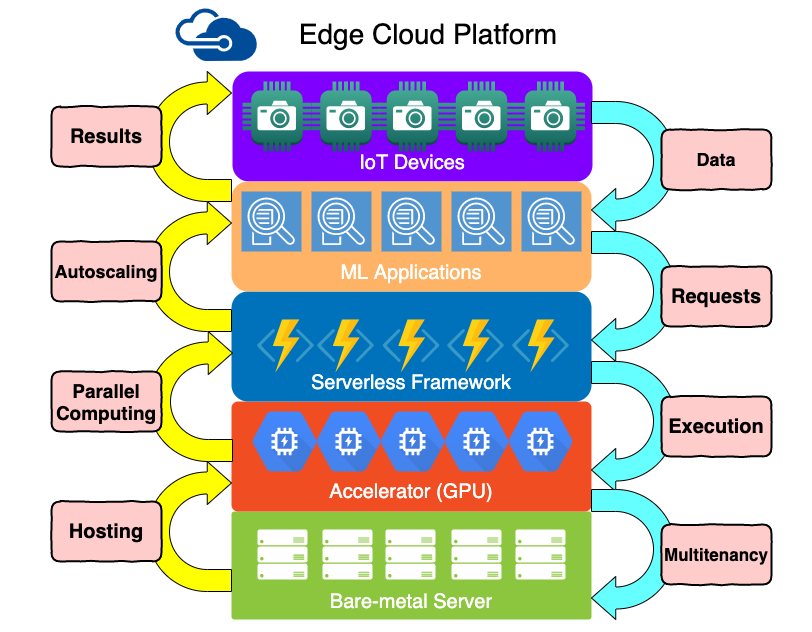
\includegraphics[scale=0.3]{figures/edge_platform}
    \caption{The abstract design of an edge cloud platform leveraging serverless framework and GPUs for executing distributed machine learning applications in IoT settings.
\label{fig:edge}}
\end{figure}

As depicted in Figure~\ref{fig:edge}, we envision an ideal edge cloud platform, to which IoT devices transmit data in batches for training and inference applications. The hierarchy of the platform has five layers: (1) \textbf{bare-metal server} cluster hosts hardware using multitenancy; (2) \textbf{accelerators} (i.e. GPUs) provide computational power by parallel computing; (3) \textbf{serverless framework} autoscales function execution upon the rate of requests; (4) \textbf{machine learning application} receives streaming data from (5) \textbf{IoT devices} and returns results (i.e. classification, regression, etc.)

In this paper, we present STOIC (Serverless TeleOperable Hybrid Cloud) that embraces such designing philosophy. Unique to STOIC, however, is its offloading system which intelligently places the application workload on edge and cloud systems based on its precise prediction of total latency. We consider three major contributions from this work: (1) we design and implement a serverless framework serving IoT requests by leveraging GPU acceleration. (2) we investigate feedback control mechanism and various analytical methodologies to precisely model the unstable edge and public cloud environments. (3) we test the efficacy of using this extended serverless model for machine learning applications that span edge-cloud systems, and empirically evaluate the performance of doing so. Using real workloads and deployments, we find that STOIC reduces the total response time of the benchmark application by 55\% (2.3x speedup), compared with baseline scenario. In the evaluation of duplicator mode, STOIC promptly responds to 95\% (2 GPUs) - 97\% (1 GPU) of requested workloads with the least latency in a 24-hour experiment. 
\fi

